% Lecture 1: the control-volume approach (a finite region; only what crosses its boundary matters)
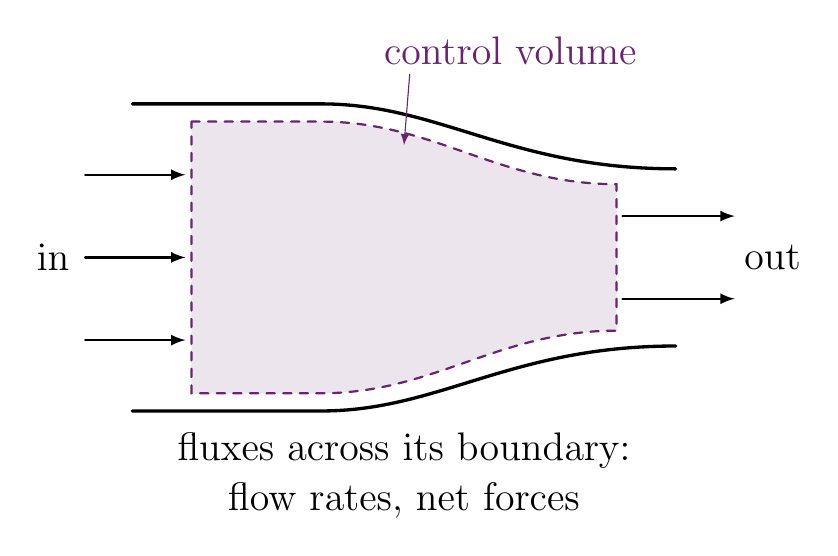
\begin{tikzpicture}[scale=1.5, >=latex, line cap=round]
  \definecolor{dpurple}{HTML}{68246D}
  % duct walls
  \draw[very thick] (0,1.3) -- (1.6,1.3) .. controls (2.6,1.3) and (3.2,0.75) .. (4.6,0.75);
  \draw[very thick] (0,-1.3) -- (1.6,-1.3) .. controls (2.6,-1.3) and (3.2,-0.75) .. (4.6,-0.75);
  % control volume
  \fill[dpurple!12] (0.5,1.15) -- (1.6,1.15) .. controls (2.55,1.15) and (3.1,0.62) .. (4.1,0.62)
                    -- (4.1,-0.62) .. controls (3.1,-0.62) and (2.55,-1.15) .. (1.6,-1.15) -- (0.5,-1.15) -- cycle;
  \draw[dpurple, thick, dashed] (0.5,1.15) -- (1.6,1.15) .. controls (2.55,1.15) and (3.1,0.62) .. (4.1,0.62)
                    -- (4.1,-0.62) .. controls (3.1,-0.62) and (2.55,-1.15) .. (1.6,-1.15) -- (0.5,-1.15) -- cycle;
  % fluxes in / out
  \foreach \y in {-0.7,0,0.7} \draw[->, thick] (-0.4,\y) -- (0.45,\y);
  \foreach \y in {-0.35,0.35} \draw[->, thick] (4.15,\y) -- (5.1,\y);
  \node[left, align=right, font=\Large] at (-0.45,0) {in};
  \node[right, font=\Large] at (5.1,0) {out};
  \node[dpurple, font=\Large] (cv) at (3.2,1.75) {control volume};
  \draw[dpurple, ->] (cv.south west) ++(0.3,0) -- (2.3,0.95);
  \node[font=\Large, align=center] at (2.3,-1.85) {fluxes across its boundary:\\ flow rates, net forces};
\end{tikzpicture}
